Unlike the analog-to-digital converter (ADC) explored in lab five, a digital-to-analog converter (DAC) attempts to take a stream of binary values and convert it into a continuous waveform.  Because there is a limited set of~$2^n$ values that can possibly be described by an~$n$-bit DAC, the resulting signal appears to be quantized as in the example in Figure~\ref{fig:theory}.
%
\begin{figure}[H]
	\centering
	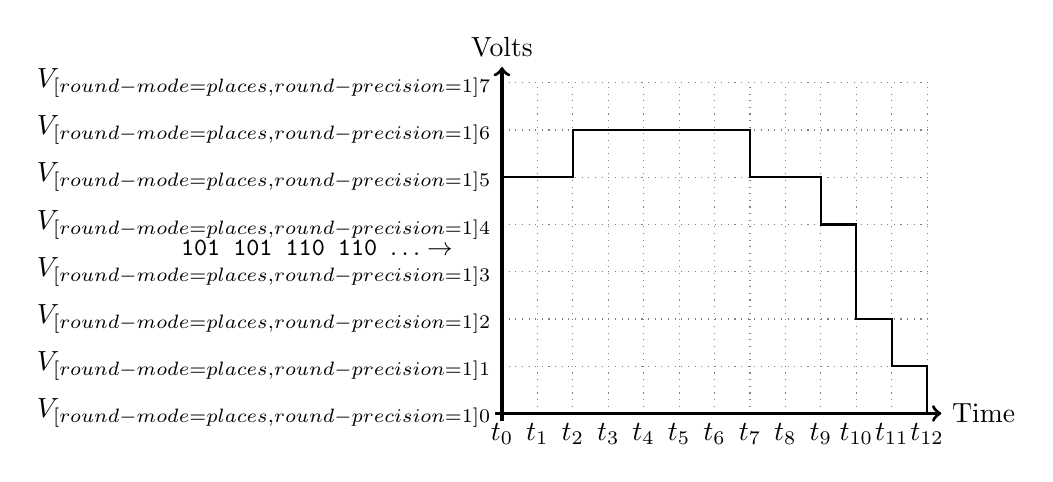
\begin{tikzpicture}[xscale=.9]
		% samples
		\draw[xstep=.5, ystep=.6, thin, color=gray, dotted] (0,0) grid (6, 4.2);

		% path
		\draw[thick]
		(0, 3)
		-- (.5, 3) -- (1, 3)
		-- (1, 3.6) -- (1.5, 3.6) -- (2, 3.6) -- (2.5, 3.6) -- (3, 3.6) -- (3.5, 3.6)
		-- (3.5, 3) -- (4, 3) -- (4.5, 3)
		-- (4.5, 2.4) -- (5, 2.4)
		-- (5, 1.2) -- (5.5, 1.2)
		-- (5.5, 0.6) -- (6.0, 0.6)
		-- (6.0, 0);

		% xtics
		\foreach \x in {0, ..., 12}
		{
			\draw ({\x/2}, 0) node[below] {$t_{\x}$};
		}

		% ytics
		\foreach \y in {0, 1, ..., 7.1}
		{
			\draw[thick] (0, .6*\y) node[left] {$V_{\num[round-mode=places, round-precision=1]{\y}}$};
		}

		% axes
    	\draw[->, very thick] (-0.1,0) -- (6.2,0) node[right] {Time};
    	\draw[->, very thick] (0,-.1) -- (0,4.4) node[above] {Volts};

		% data input
		\draw
		(0, 2.1) node[left=.5cm]{\texttt{\small 101 101 110 110 $\ldots \rightarrow$}};
\end{tikzpicture}

	\parbox{.6\textwidth}{
	\caption[Theory Plot]{Theoretical input and output for a~3-bit digital-to-analog converter.  Note that while the output is a sequence of discrete values, they form an analog voltage signal.}
	\label{fig:theory}}
\end{figure}
%
While the output signal is not continuous as a~``traditional'' analog signal would be, it is still considered analog because of its varying voltage.  Additionally, consider the case of a higher-quality DAC with faster clock frequency and higher resolution.  As the difference between any two time steps~$t_i$ and~$T_{i+1}$ approaches zero and the difference between any two voltages~$V_i$ and~$V_{i+1}$ approaches zero, the output more greatly resembles a continuous and~``traditional'' analog signal.

As with the ADC, a pre-constructed DAC circuit was provided to students in order to simplify the process of exploring the properties of such a system.  A schematic for the pre-built DAC is shown below in Figure~\ref{fig:dacSchem}.
%
\begin{figure}[H]
	\centering
	\begin{circuitikz}
	% body
	\draw[ultra thick] (-2, -4) rectangle (2, 4);

	% chip name
	\draw (0,0) node[rotate=90] {DAC0808};

	% -------------------- top --------------------
	\draw
	(0, 4) node[above left] {13} node[below] {$V_\text{CC}$}
		to [short, -o] ++(0, 1) node[above] {+\SI{5}{\volt}};


	% -------------------- left pins --------------------

	% resistors, LEDs, and pin ames
	\foreach \y in {7, ..., 0}
	{
		\draw (-2, \y-3.5) node[right] (b\y) {B\y}
		to [short, -o] ++(-0.5, 0);
	}

	% pin numbers
	\foreach \pin in {5,...,12}
	{
		\draw (-2, 8.5-\pin) node[above left] {\pin};
	}

	% LSB and MSB
	\draw (b7) node[right=4.5pt] {(MSB)}
	(b0) node[right=4.5pt] {(LSB)};

	% digital inputs label
	\path[draw, text centered ] (-3, 4) -- node[rectangle, fill=white, rotate=90] {Digital Inputs} (-3, -4);
	\draw
	(-3, 4)  -- ++(.5, 0)
	(-3, -4) -- ++(.5, 0);

	% -------------------- right pins --------------------

	% Vee and cap
	\draw
	(0, -4) node[below right] {3} node[above]{$V_\text{EE}$}
		to [short, -o] ++(0, -1.5) node[below] {\SI{-15}{\volt}}
	(2, -3.5) node[above right] {16} to [short] ++(1, 0) to [C, l=\SI{0.1}{\micro\farad}] ++(0, -1.5)
		to [short] ++(-3, 0);

	% pin 4
	\draw
	(2, -1) node[above right] {4} to [short] ++(1, 0)
		to [R, l=\SI{5}{\kilo\ohm}] ++(0, -1.5) node[ground] {}
	(3.5, -1) node[right] {$V_0$} to [short, i_=$I_0$, o-] ++(-.5, 0);

	% pins 15 & 2
	\draw
	(2, .5) node[above right] {2} to [short] ++(2.5, 0) node[ground] {}
		to [short] ++(0, 1)
	(2, 1.5) node[above right] {15} to [short] ++(.5, 0)
		to [R, l=\SI{5}{\kilo\ohm}] ++(2, 0);

	% pins 14
	\draw
	(2, 3.5) node[above right] {14} node[left] {$V_\text{REF}$} to [short] ++(.5, 0)
		to [R, l=\SI{5}{\kilo\ohm}, -o] ++(2, 0) node[below] {+\SI{5}{\volt}};


	% = - V_\text{REF} \left( \frac{A_1}{2} + \frac{A_2}{4} + \ldots + \frac{A_8}{256} \right)$}
\end{circuitikz}

	\parbox{.6\textwidth}{
	\caption[Digital-to-Analog IC schematic]{Circuit schematic provided in the
	lab instructions, describing the layout of the pre-built circuit used in
	experiment six.}
	\label{fig:dacSchem}}
\end{figure}
%
To make the process even simpler for students, the digital inputs were wired directly to the corresponding bits of a known-working ADC, such as the one used in the previous week.  Since every other pin has been properly connected, students must only focus on the voltage that appears at pin~4.  Note that because of the configuration of the~\SI{5}{\kilo\ohm} resistor, the output voltage will always be negative, as given in the lab instructions by~\eqref{eq:vout}:
%
\begin{equation}
	V_\text{out} = - V_\text{REF} \left( \frac{A_0}{2} + \frac{A_1}{4} + \ldots + \frac{A_7}{256} \right) \quad \text{,}
	\label{eq:vout}
\end{equation}
%
where~$A_0$ through~$A_7$ represent the eight bits of input to the DAC.  Regardless, pin four was wired directly to an input of an oscilloscope was measured throughout the experiment.
